%!TEX root = ../template.tex
%%%%%%%%%%%%%%%%%%%%%%%%%%%%%%%%%%%%%%%%%%%%%%%%%%%%%%%%%%%%%%%%%%%%
%% chapter4.tex
%% NOVA thesis document file
%%
%% Chapter with lots of dummy text
%%%%%%%%%%%%%%%%%%%%%%%%%%%%%%%%%%%%%%%%%%%%%%%%%%%%%%%%%%%%%%%%%%%%

\typeout{NT FILE chapter4.tex}%

\chapter{Results}
\label{cha:results}

\section{Evaluation Methodology} % (fold)
\label{sec:evaluation_methodology}

\paragraph{Environment}

The experiments were conducted in a cloud environment with 10 virtual machines.
All 10 nodes were hosted in the same datacenter in the region of Strasbourg, France.
Each virtual machines was hosted in different physical machines, no two VMs shared the same hardware.
Each node is interconnected with a bandwidth of 2 Gb/s.
Each virtual machine is equipped with 4GB of RAM and 2 virtual cores of an Intel Core Haswell (no TSX) cpu.

\paragraph{Tested microservice system }

To test the cost of the adapter system a demo application was developed.
The demo application holds a configurable amount of services that run an identical image.
The image is a simple http spring server that returns received requests unchanged.
The interconnections between microservices is configurable thorough environment variables.
The number of synchronous calls (SyC) between microservices for a single request is also configurable.
The number of parallel calls (PrC) between microservices is also configurable.
Two http endpoints are contained in the image, which was developed in two separate versions with unique contracts.
In one of the endpoints, all the parameters in the body's schema were given new names.

\paragraph{Experiment Setup}

To inject load in the experiments, 10 workers of artillery load testing tool were used,
the workers are executed remotely in the cluster and were spread in 6 nodes.
The workers are supported by kubernetes pods that are monitored by a common kubernetes job.
The workers are installed and removed from cluster using the artillery operator project, that enables
the creation and execution of distributed Artillery load tests from a Kubernetes cluster, at scale.
In each experiment all the resources of previous experiments were deleted and a new job and namespace were created in the
cluster to avoid contamination in the metrics extracted.
Each experiment was executed in sequence with an pause of 2m.

Each experiment had three phases:
A warm up phase of 30s with an arrival rate of 5 vu/s.
A ramp up phase of 2m.
A sustained load phase of 6m.
The metrics were only extracted during the sustained load phase;
the first and last 30s were left out to allow time for all the artillery worker threads to enter the sustained load phase.
We excluded results from experiments that had a high enough throughput to saturate the application.
The error rate and timeouts were zero during all the presented experiments.

\begin{figure}[htbp]
    \centering
    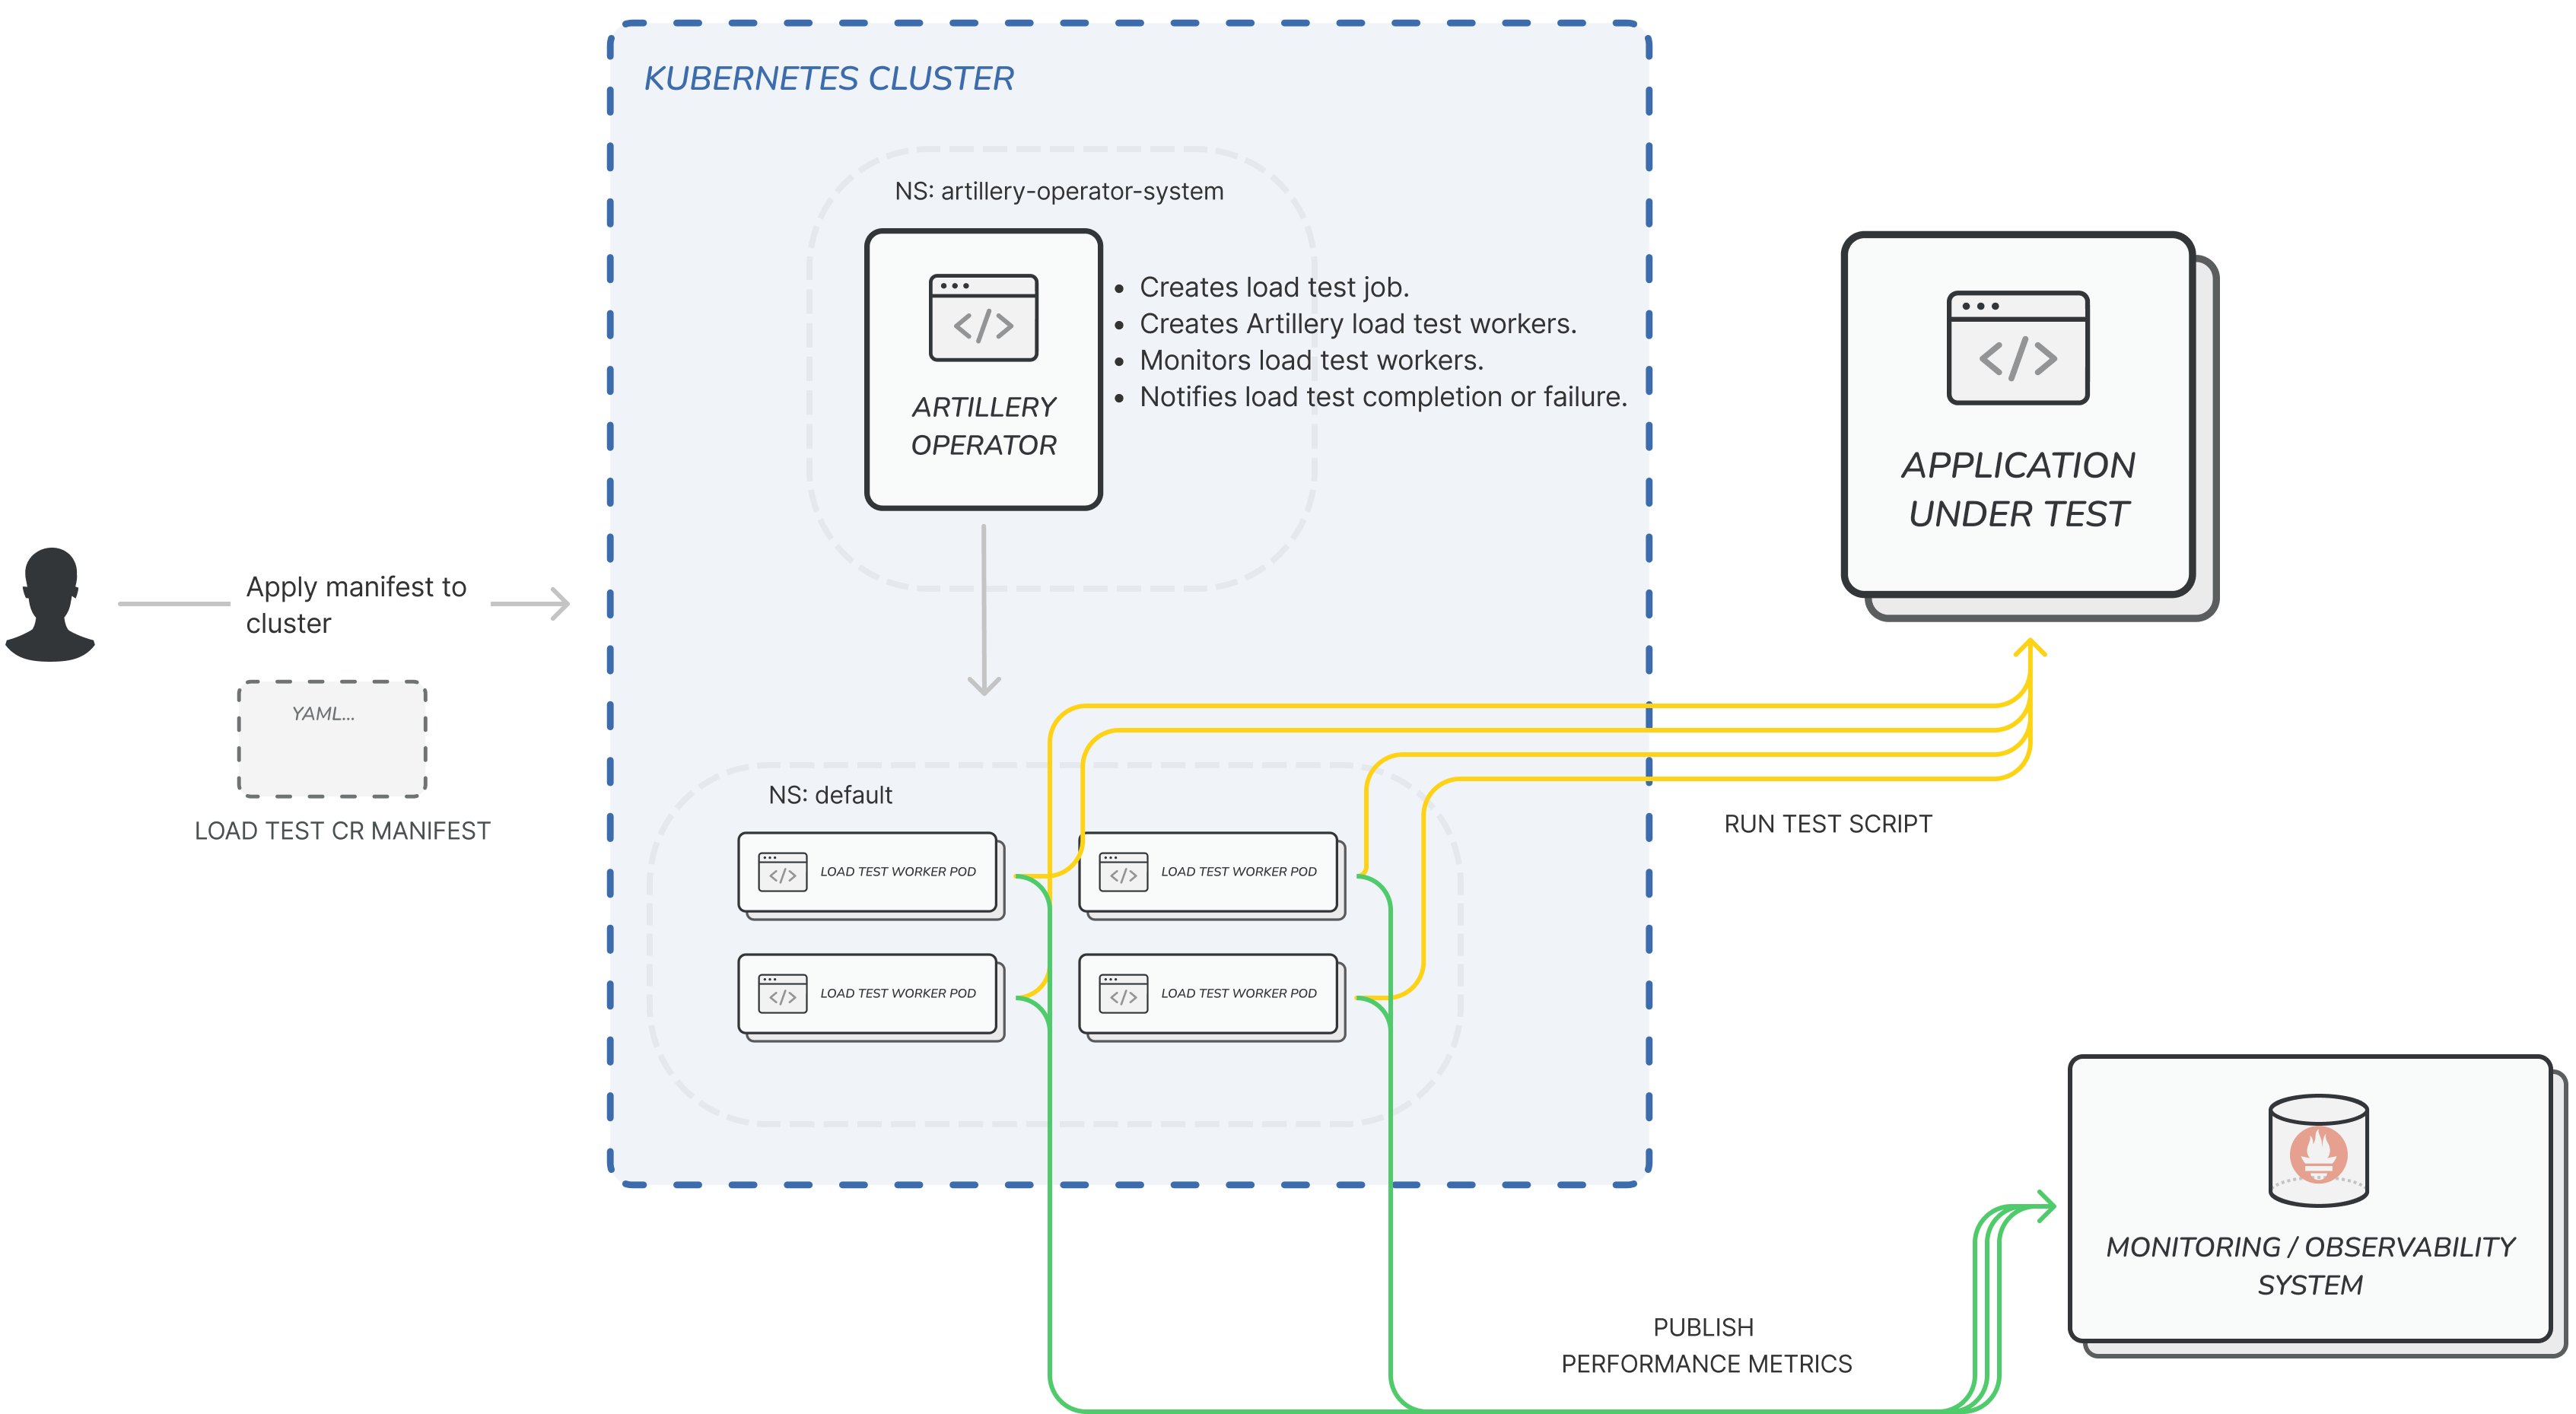
\includegraphics[height=3in]{artillery-operator-architecture}
    \caption{Artillery Operator Architecture}
    \label{fig:gantt}
\end{figure}

\paragraph{Metrics}

In each experiment we extracted 4 metrics, the cpu/memory resources and the throughput and latency of the system.
The resources were only queried from the adapters, and the replicas that belong to the target microservice application.
The resources consumed by the monitoring system and artillery workers were excluded and have no effect
on the results.
The throughput and latency were extracted with the use of the artillery load testing tool.

The cpu resources samples were extracted with an interval of 5 seg from each node using prometheus node exporter.
The memory resources samples were extracted with an interval of 5 seg from each container using kubelet node agent api.
The throughput and latency statistics were calculated with a period of 10s over 5 min, the results obtained represent the
average of the reported 30 periods.

\section{Experiments} % (fold)
\label{sec:experiments}

%%Throughout the experiments, if the behavior of the system is similar with different parameters, we select the most
%%interesting figures or features due to the limited space.

\subsection{Point to Point} % (fold)
\label{sec:point to point}

\begin{figure}[htbp]
    \centering
    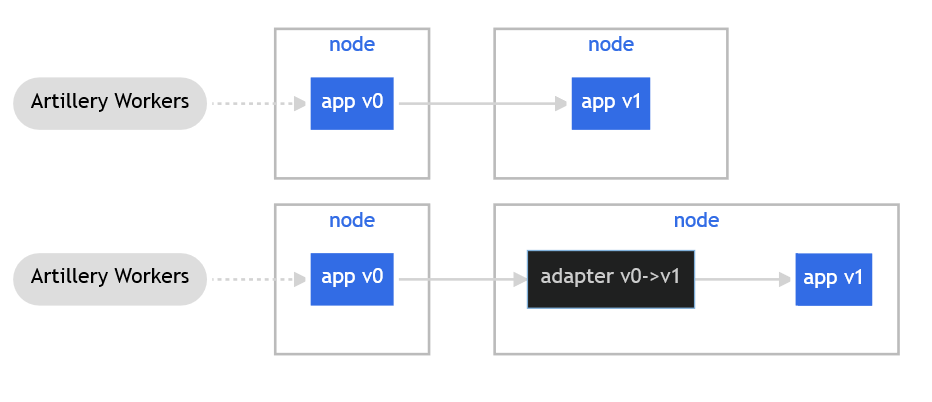
\includegraphics[height=2.4in]{pointExperiment}
    \caption{point-to-point experiment}
    \label{fig:gantt}
\end{figure}


\begin{figure}[htbp]
    \centering
    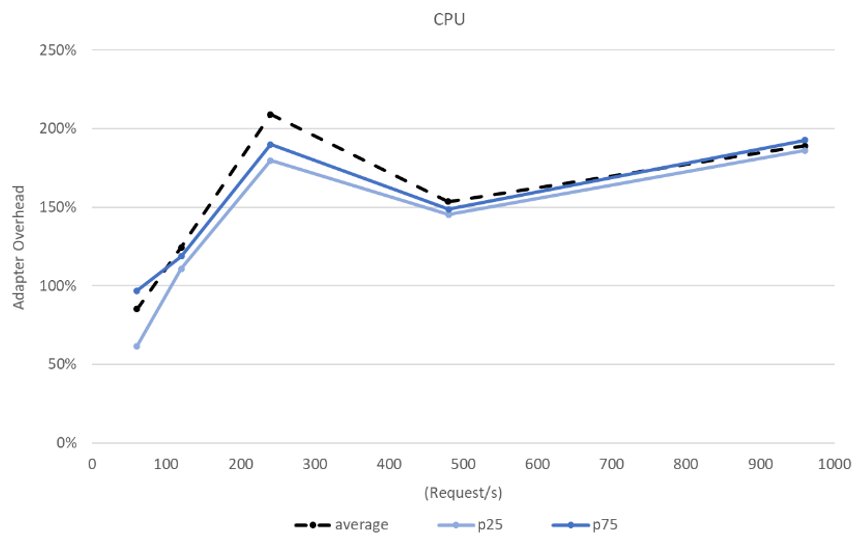
\includegraphics[height=3in]{Results/PtP/Cpu-PtP}
    \label{fig:gantt}
\end{figure}

\begin{figure}[htbp]
    \centering
    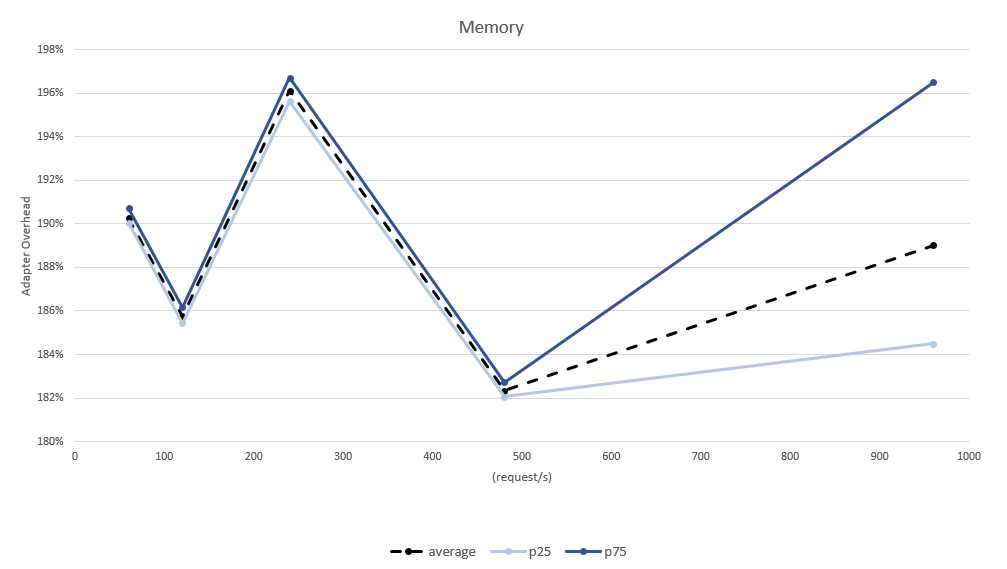
\includegraphics[height=3in]{Results/PtP/Memory-PtP}
    \label{fig:gantt}
\end{figure}

\begin{figure}[htbp]
    \centering
    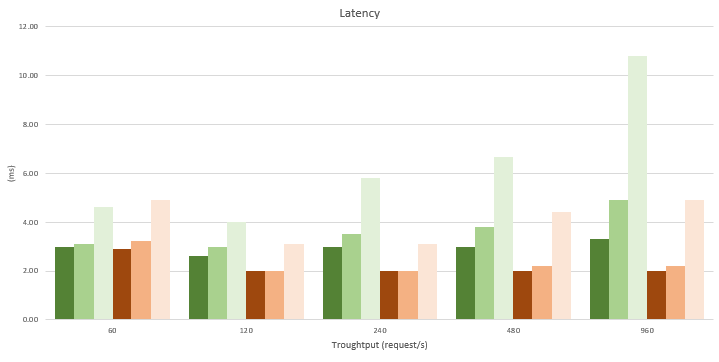
\includegraphics[height=3in]{Results/PtP/Latency-PtP}
    \label{fig:gantt}
\end{figure}

\begin{figure}[htbp]
    \centering
    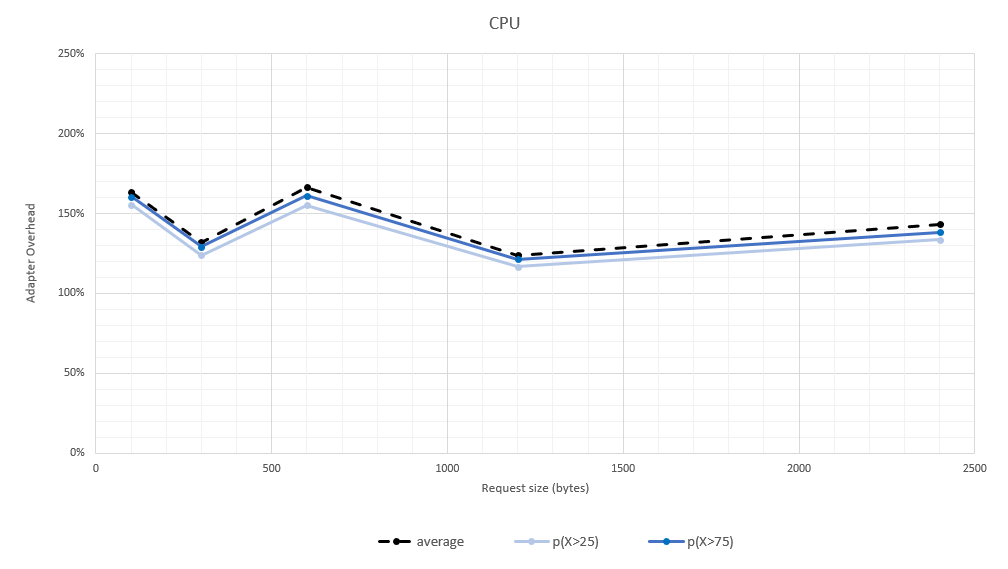
\includegraphics[height=3in]{Results/PtP_Size/Cpu-PtP_Size}
    \label{fig:gantt}
\end{figure}

\begin{figure}[htbp]
    \centering
    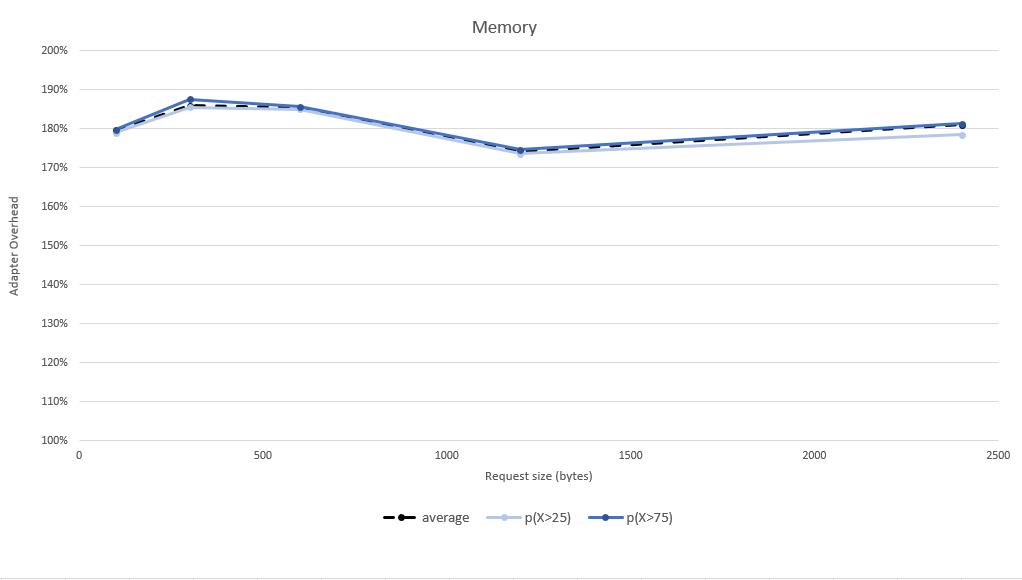
\includegraphics[height=3in]{Results/PtP_Size/Memory-PtP_Size}
    \label{fig:gantt}
\end{figure}

\begin{figure}[htbp]
    \centering
    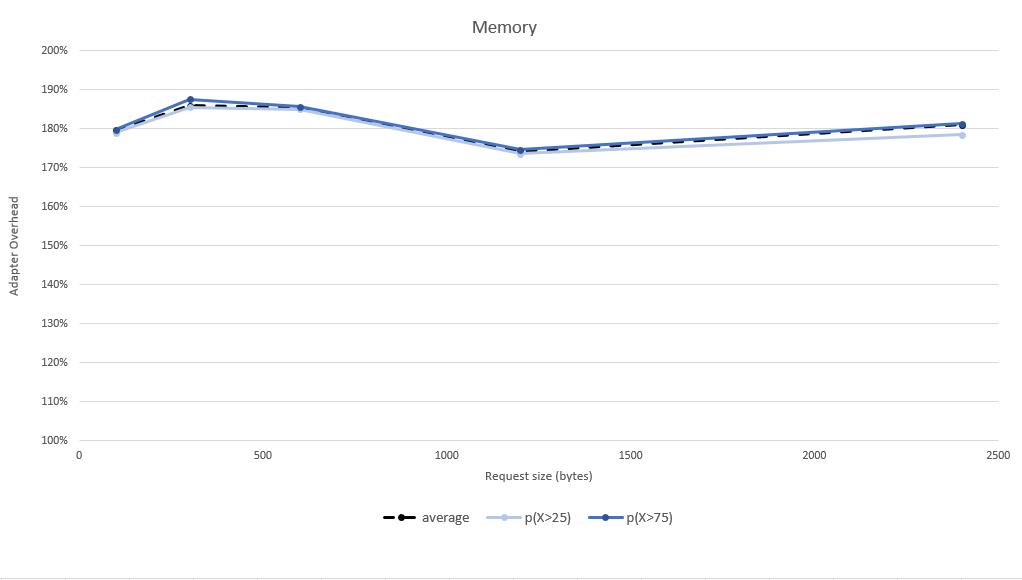
\includegraphics[height=3in]{Results/PtP_Size/Latency-PtP_Size}
    \label{fig:gantt}
\end{figure}

\begin{figure}[htbp]
    \centering
    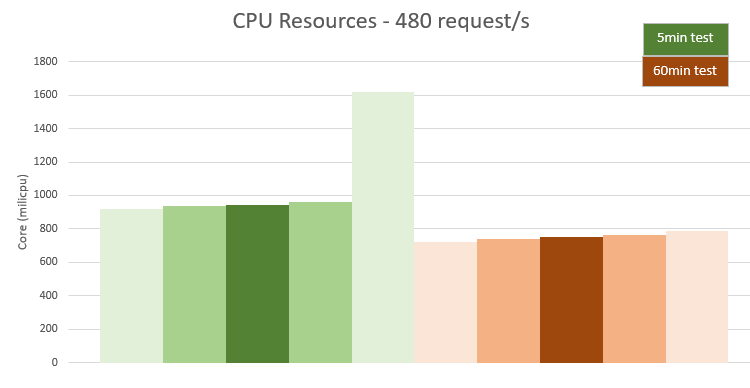
\includegraphics[height=3in]{Results/Ls/Cpu-Ls}
    \label{fig:gantt}
\end{figure}

\begin{figure}[htbp]
    \centering
    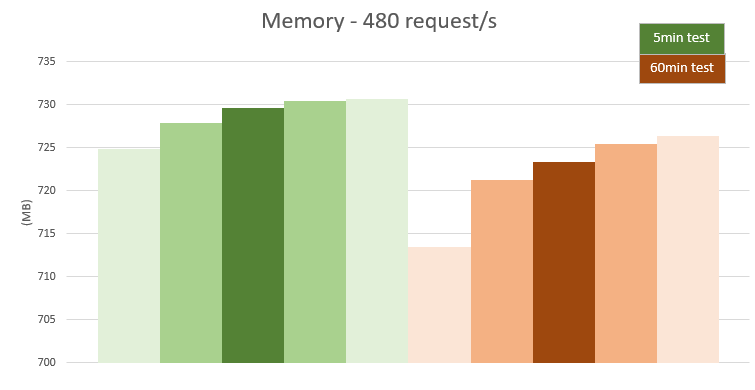
\includegraphics[height=3in]{Results/Ls/Memory-Ls}
    \label{fig:gantt}
\end{figure}

\begin{figure}[htbp]
    \centering
    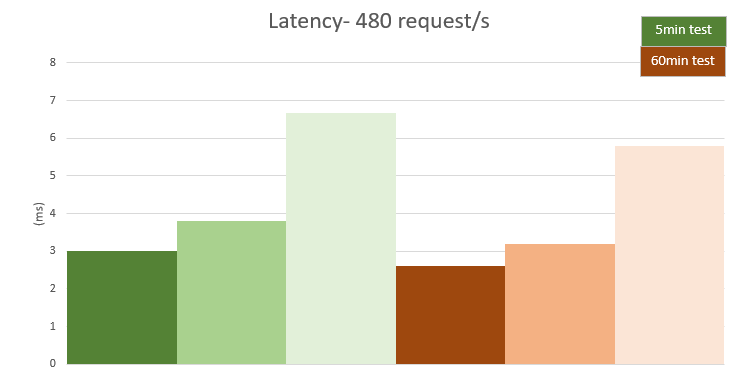
\includegraphics[height=3in]{Results/Ls/Latency-Ls}
    \label{fig:gantt}
\end{figure}

\newpage



\subsection{Weighted Point to Point} % (fold)
\label{sec:weighted point to point}

\begin{figure}[htbp]
    \centering
    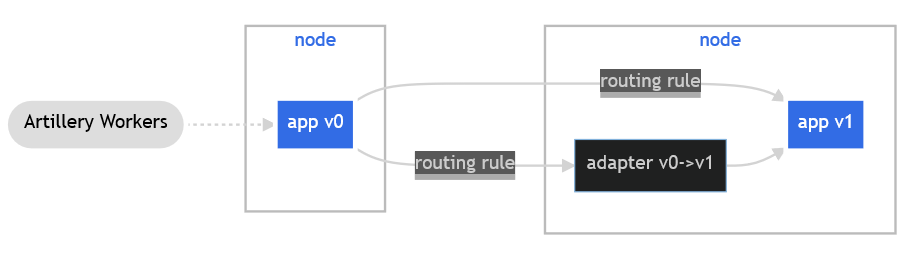
\includegraphics[height=1.8in]{routingExperiment}
    \caption{routing experiment}
    \label{fig:gantt}
\end{figure}

\begin{figure}[htbp]
    \centering
    \includegraphics[height=3in]{Results/R/Cpu-R}
    \label{fig:gantt}
\end{figure}

\begin{figure}[htbp]
    \centering
    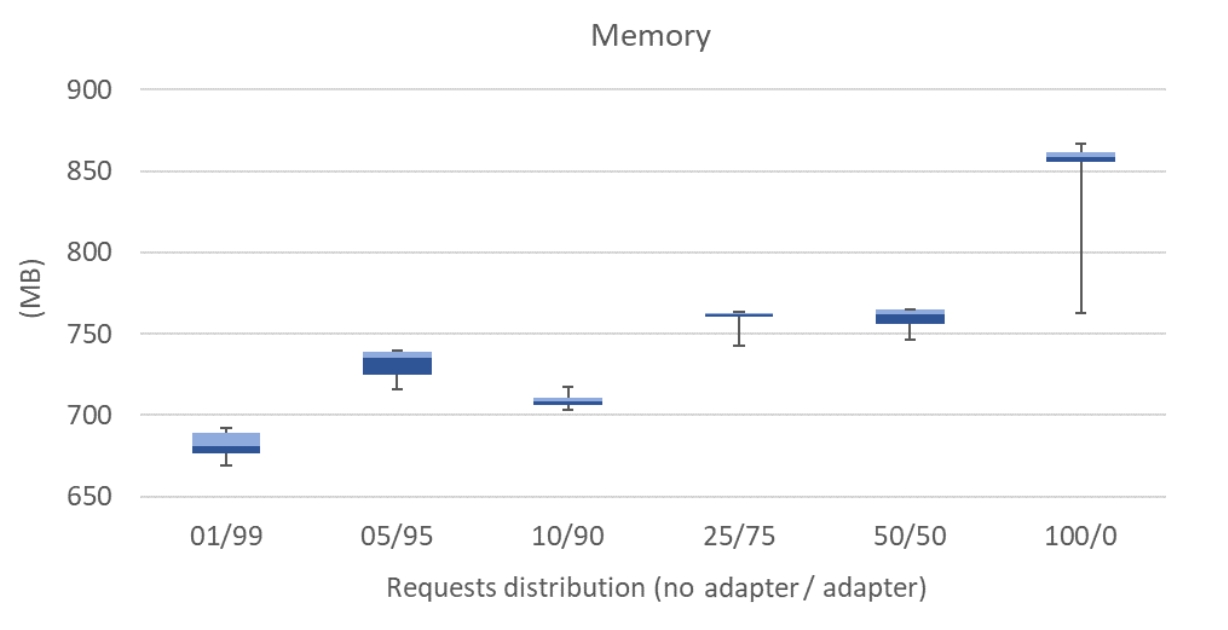
\includegraphics[height=3in]{Results/R/Memory-R}
    \label{fig:gantt}
\end{figure}

\begin{figure}[htbp]
    \centering
    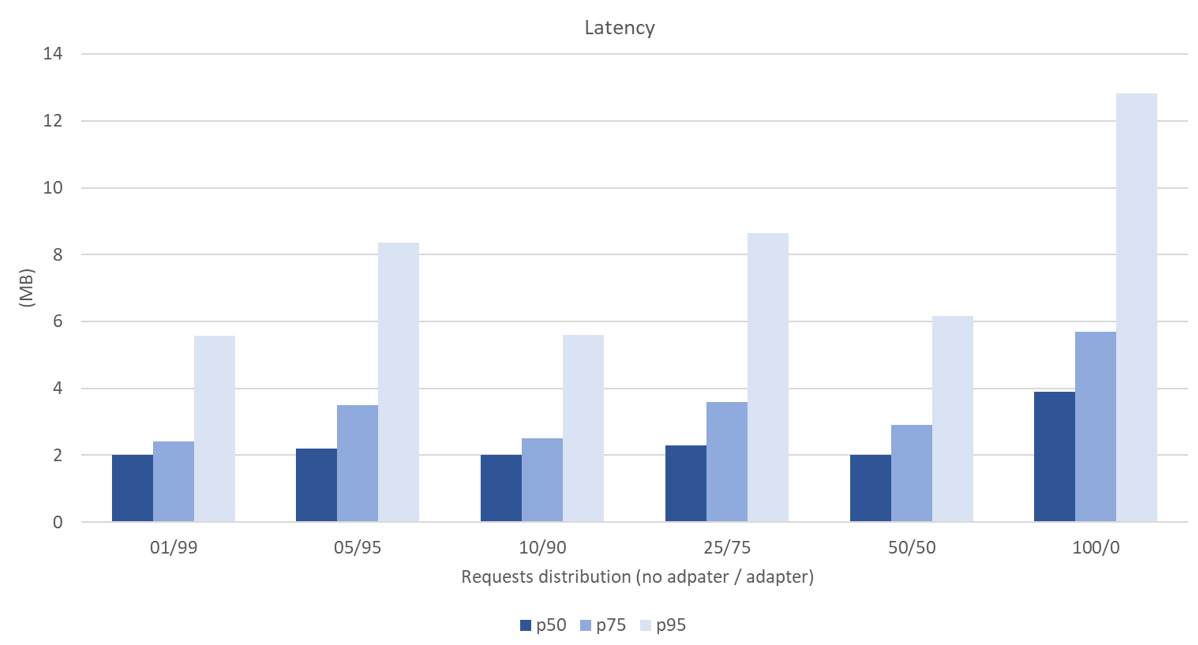
\includegraphics[height=3in]{Results/R/Latency-R}
    \label{fig:gantt}
\end{figure}

\newpage



\subsection{Bi-partition} % (fold)
\label{sec:bi-partition}

\begin{figure}[htbp]
    \centering
    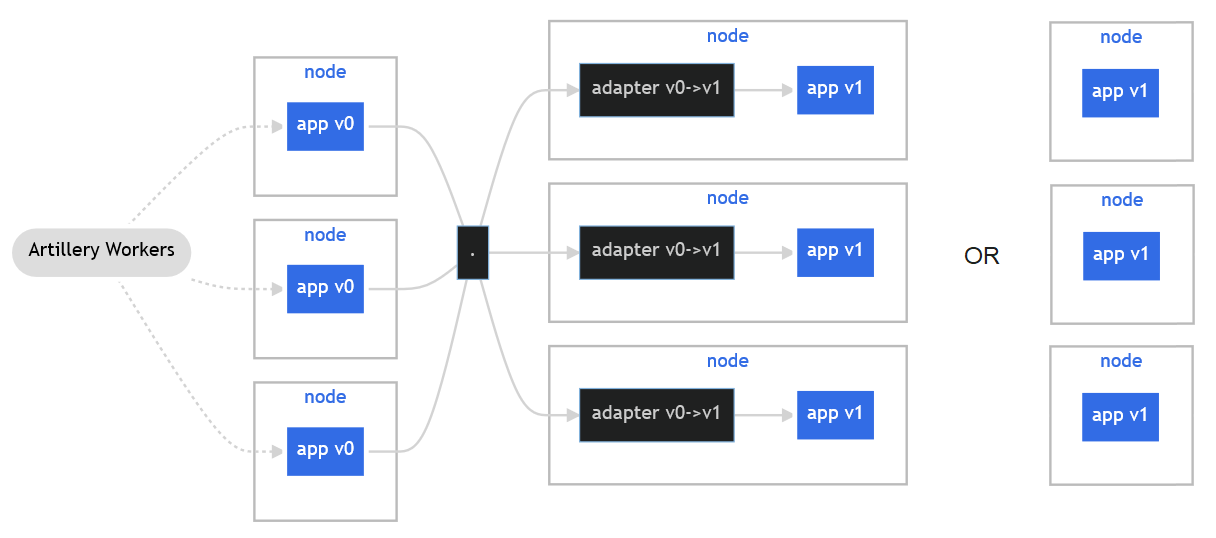
\includegraphics[height=2.7in]{bipartExperiment}
    \caption{bi-partition experiment}
    \label{fig:gantt}
\end{figure}

\begin{figure}[htbp]
    \centering
    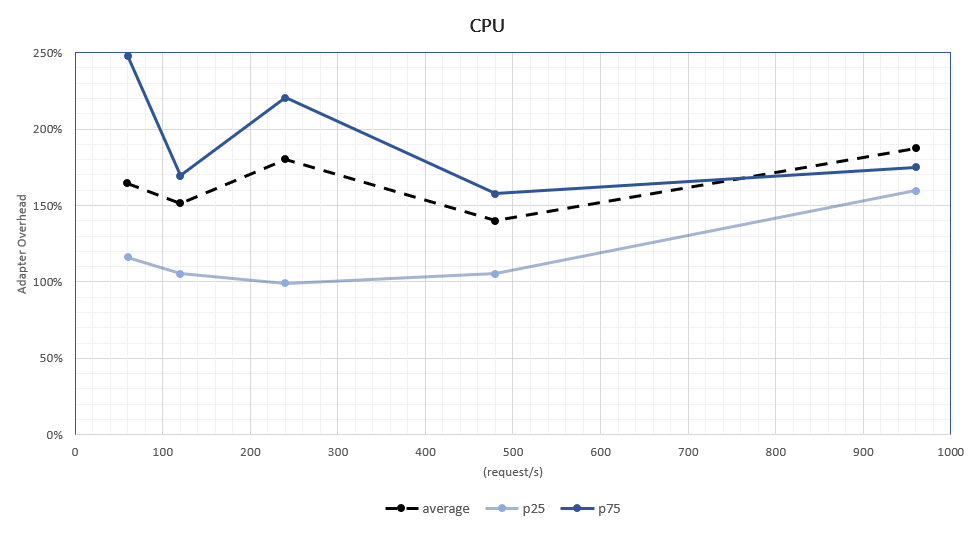
\includegraphics[height=4in]{Results/Bp/Cpu-Bp}
    \label{fig:gantt}
\end{figure}

\begin{figure}[htbp]
    \centering
    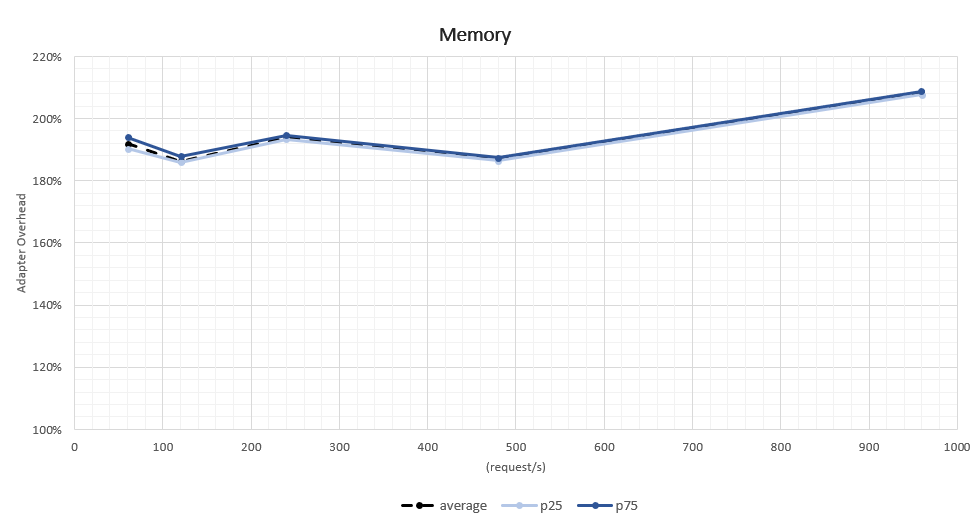
\includegraphics[height=4in]{Results/Bp/Memory-Bp}
    \label{fig:gantt}
\end{figure}

\begin{figure}[htbp]
    \centering
    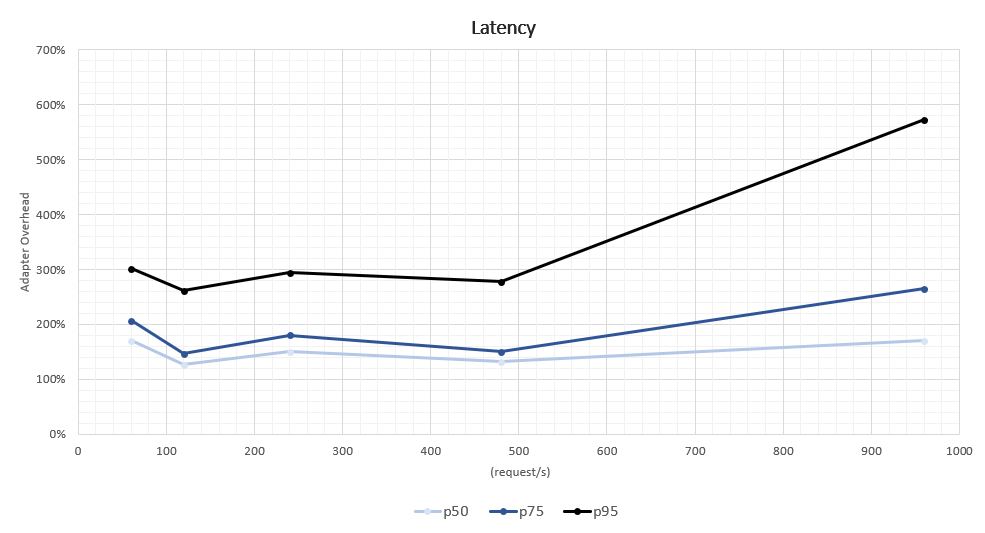
\includegraphics[height=3in]{Results/Bp/Latency-Bp}
    \label{fig:gantt}
\end{figure}

\section{Conclusions} % (fold)
\label{sec:conclusions}